% GAUSSIAN FITTING
Next, we consider the problem of fitting both the unknown mean \(\mu\) and the standard deviation \(\sigma\) of a Gaussian distribution \(\mathcal{N}(y_i \cond \mu,\sigma^2)\).
A number of independent samples \(y_i\) with \(i = 1,\ldots,\dimData\) from the normal distribution constitute the available data \(\bm{y} = (y_1,\ldots,y_\dimData)^\top\).
The data model for this situation is written as
\begin{equation} \label{eq:JCP:Normal:Data}
  \bm{Y} \cond \mu,\sigma \sim \prod\limits_{i=1}^\dimData \mathcal{N}(y_i \cond \mu,\sigma^2).
\end{equation}
% POSTERIOR DISTRIBUTION
For the likelihood function one then has \(\mathcal{L}(\mu,\sigma) = \prod_{i=1}^{\dimData} \mathcal{N}(y_i \cond \mu,\sigma^2)\).
Given a Bayesian prior \(\pi(\mu,\sigma)\), the posterior distribution is \(\pi(\mu,\sigma \cond \bm{y}) = \scale^{-1} \mathcal{L}(\mu,\sigma) \pi(\mu,\sigma)\).
This distribution aggregates the information about the two unknowns after the data have been analyzed.
\par % EXPERIMENTAL SETUP
The true values of the mean and standard deviation are set as \(\mu = 30\) and \(\sigma = 5\), respectively.
These values are treated as unknowns in the further course of the computer experiment.
We consider a situation where \(\dimData = 10\) samples are randomly drawn from the distribution in \cref{eq:JCP:Normal:Data}.
The pseudo-random numbers \(\bm{y} = (31.23,27.50,24.91,25.99,32.88,36.41,27.81,25.19,37.96,34.84)^\top\) are used as synthetic data.
We consider an independent prior \(\pi(\mu,\sigma) = \pi(\mu) \pi(\sigma)\) with uniform marginals
\(\pi(\mu) = \mathcal{U}(\mu \cond \underline{\mu},\overline{\mu})\) and \(\pi(\sigma) = \mathcal{U}(\sigma \cond \underline{\sigma},\overline{\sigma})\)
over bounded supports \(\mathcal{D}_{\mu} = [\underline{\mu},\overline{\mu}] = [20,40]\) and \(\mathcal{D}_{\sigma} = [\underline{\sigma},\overline{\sigma}] = [2,10]\).
As opposed to the conjugate example above, this two-dimensional model does not permit a closed-form expression of the posterior density and the model evidence.

\subsubsection{Posterior density}
% LIKELIHOOD EXPANSION
Now we proceed analogously to the investigation of the normal model with known variance.
Expansions \(\hat{\mathcal{L}}_p\) of the likelihood \(\mathcal{L}\) are computed and contrasted for different experimental designs of size \(K\) and different polynomial orders \(p\).
An appropriate linear transformation to uniform standardized variables is applied such that the unknowns are represented as
\(\mu = (\overline{\mu} - \underline{\mu}) / 2 \cdot \xi_{\mu} + (\underline{\mu} + \overline{\mu}) / 2\) and 
\(\sigma = (\overline{\sigma} - \underline{\sigma}) / 2 \cdot \xi_{\sigma} + (\underline{\sigma} + \overline{\sigma}) / 2\), respectively.
Here, \(\xi_{\mu},\xi_{\sigma} \in [-1,1]\) are the corresponding standardized variables with a uniform weight function.
Accordingly, tensorized Legendre polynomials form the trial basis.
Two-dimensional Sobol sequences are utilized as uniformly space-filling experimental designs.
\par % SLE CONVERGENCE
As before, the speed of convergence and the prediction accuracy of the SLE are analyzed first.
The normalized empirical error \(\epsilon_{\mathrm{Emp}}\) and the normalized LOO error \(\epsilon_{\mathrm{LOO}}\) are therefore monitored throughout a series of runs that are conducted
for an experimental design of the fixed size \(K = 1 \times 10^5\) and for an increasing expansion order up to \(p = 50\).
In \cref{fig:JCP:Normal:ConvSLE} a corresponding plot is shown, where the convergence of the SLE  \(\hat{\mathcal{L}}_p\) to the likelihood function \(\mathcal{L}\) is diagnosed.
The reason that \(\epsilon_{\mathrm{Emp}}\) and \(\epsilon_{\mathrm{LOO}}\) do not significantly differ is that the large size of the experimental design prevents overfitting.
For \(p = 50\) the normalized empirical error and the normalized LOO error are found as \(\epsilon_{\mathrm{Emp}} = 5.56 \times 10^{-11}\)
and \(\epsilon_{\mathrm{LOO}} = 6.05 \times 10^{-11}\), respectively.
This shows that the likelihood function \(\mathcal{L}\) can be indeed expanded in the Legendre basis.
For the uniform prior distribution that is used here, the normalized SLE errors effectively measure the errors of the posterior density.
% FIGURE: SLE CONVERGENCE
\begin{figure}[htbp]
  \centering
  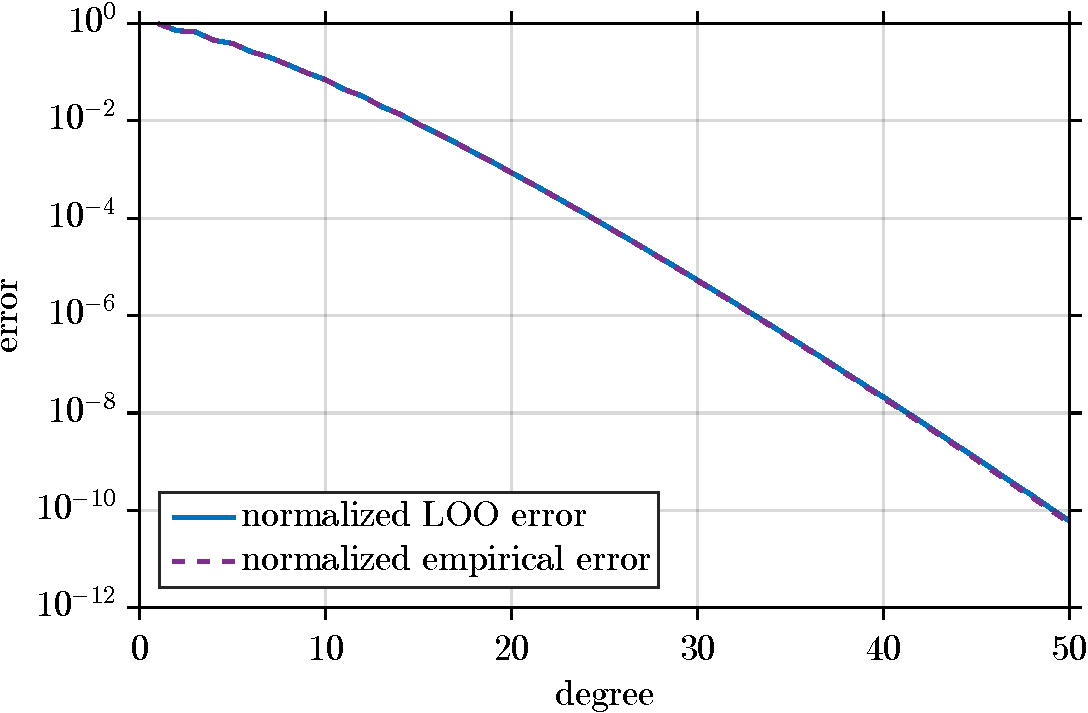
\includegraphics[height=\JCPfigHeight]{fig_JCP_Norm2D_ConvSLE}
  \caption[2D normal fitting: Convergence of the SLE]{2D normal fitting: Convergence of the SLE.}
  \label{fig:JCP:Normal:ConvSLE}
\end{figure}
\par % POSTERIOR DENSITY
Now the joint posterior density \(\pi(\mu,\sigma \cond \bm{y})\) is computed and plotted in \cref{fig:JCP:Normal:Post2D}.
For comparison purposes the posterior is sampled by means of MCMC simulation first.
A simple random walk Metropolis (RWM) sampler with a Gaussian instrumental distribution is utilized.
With this algorithm an unusually large number of \(10^7\) MCMC samples is drawn from the posterior.
This serves the purpose of providing very accurate results that act as references for the SLE-based estimates.
In \cref{fig:JCP:Normal:Post2D:MCMC} a normalized histogram of the obtained RWM sample is shown.
Next, the joint posterior density \(\pi(\mu,\sigma \cond \bm{y}) \approx \coeffL_{\bm{0}}^{-1} \hat{\mathcal{L}}_p(\mu,\sigma) \pi(\mu,\sigma)\)
is computed via \cref{eq:JCP:SLE:Posterior,eq:JCP:SLE:ScaleFactor}.
The SLE \(\hat{\mathcal{L}}_p(\mu,\sigma)\) with \(p = 50\) that features the lowest LOO error is used.
In \cref{fig:JCP:Normal:Post2D:SLE} the posterior surrogate that arises from the SLE is plotted.
For a later comparison with the heat conduction example,
in \cref{fig:JCP:Normal:Post3D:SLE} the SLE posterior surrogate from \cref{fig:JCP:Normal:Post2D:SLE} is plotted again from a different angle.
By visual inspection the obvious similarity between the density \(\pi(\mu,\sigma \cond \bm{y})\) sampled by MCMC and emulated by the SLE is noticed.
% FIGURES: 2D POSTERIORS
\begin{figure}[htbp]
  \centering
  \begin{subfigure}[b]{\JCPsubWidth}
    \centering
    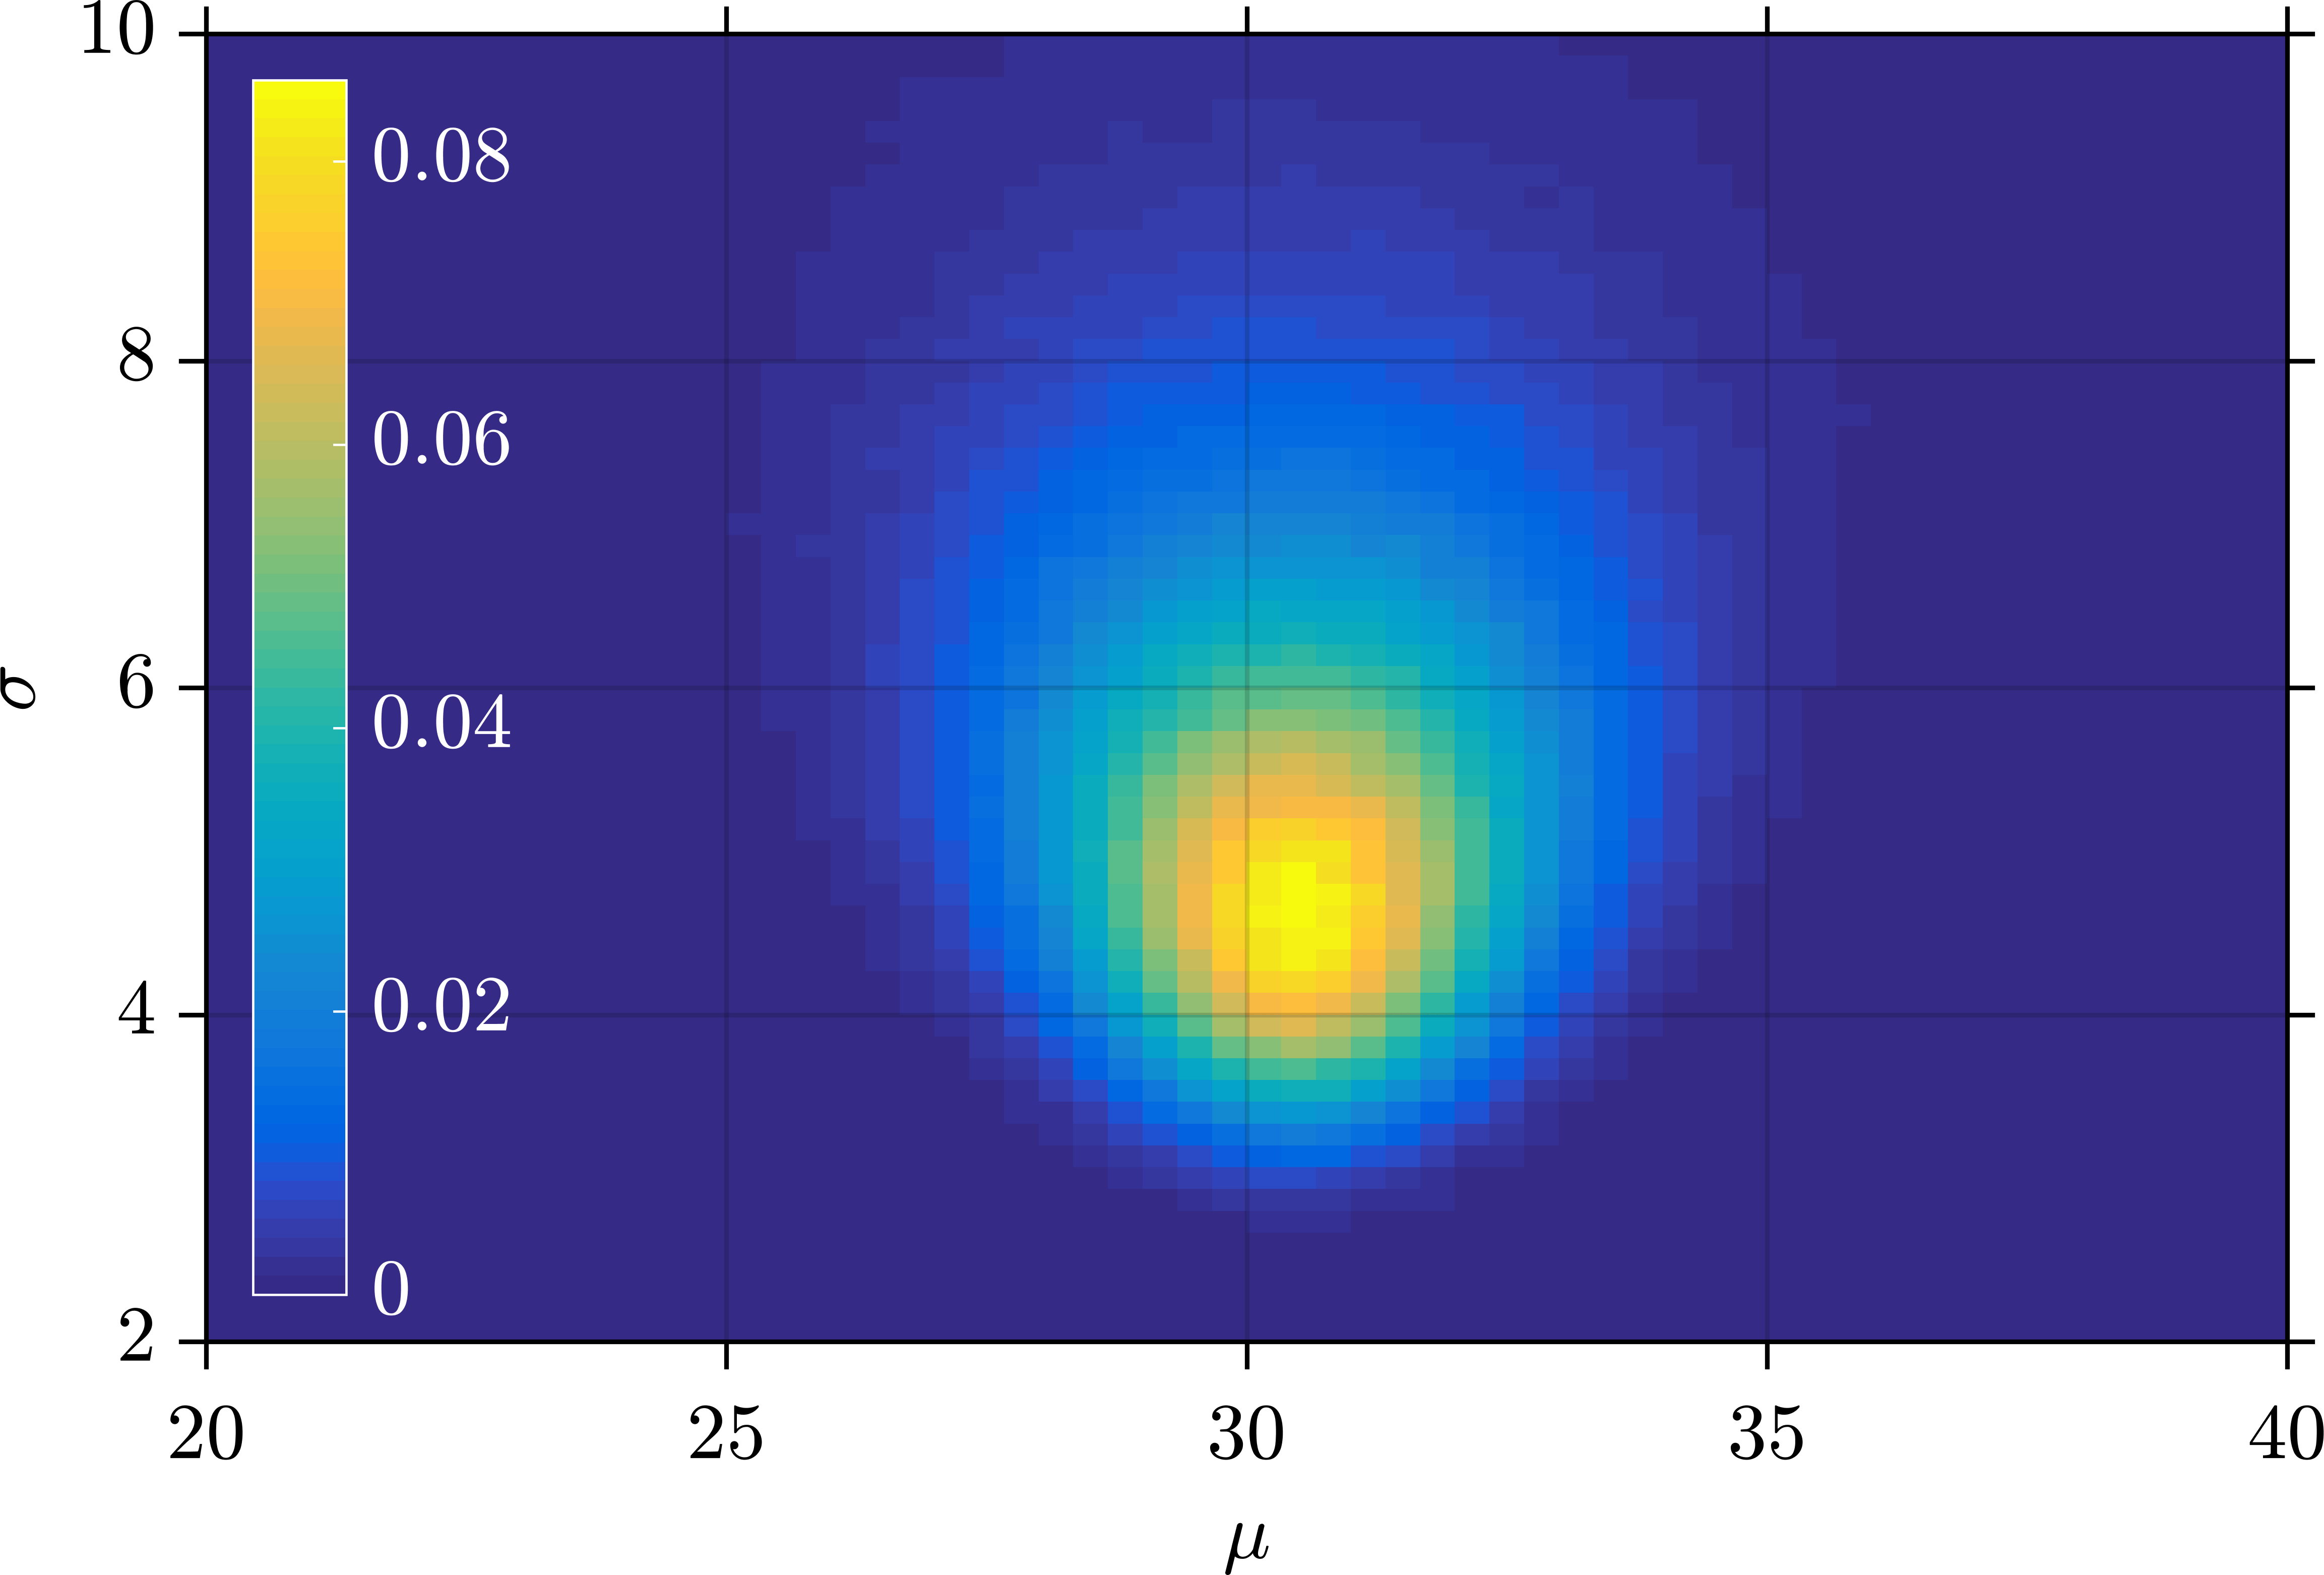
\includegraphics[height=\JCPfigHeight]{fig_JCP_Norm2D_Post2D_MCMC}
    \caption{MCMC reference sample.}
    \label{fig:JCP:Normal:Post2D:MCMC}
  \end{subfigure}\hfill%
  \begin{subfigure}[b]{\JCPsubWidth}
    \centering
    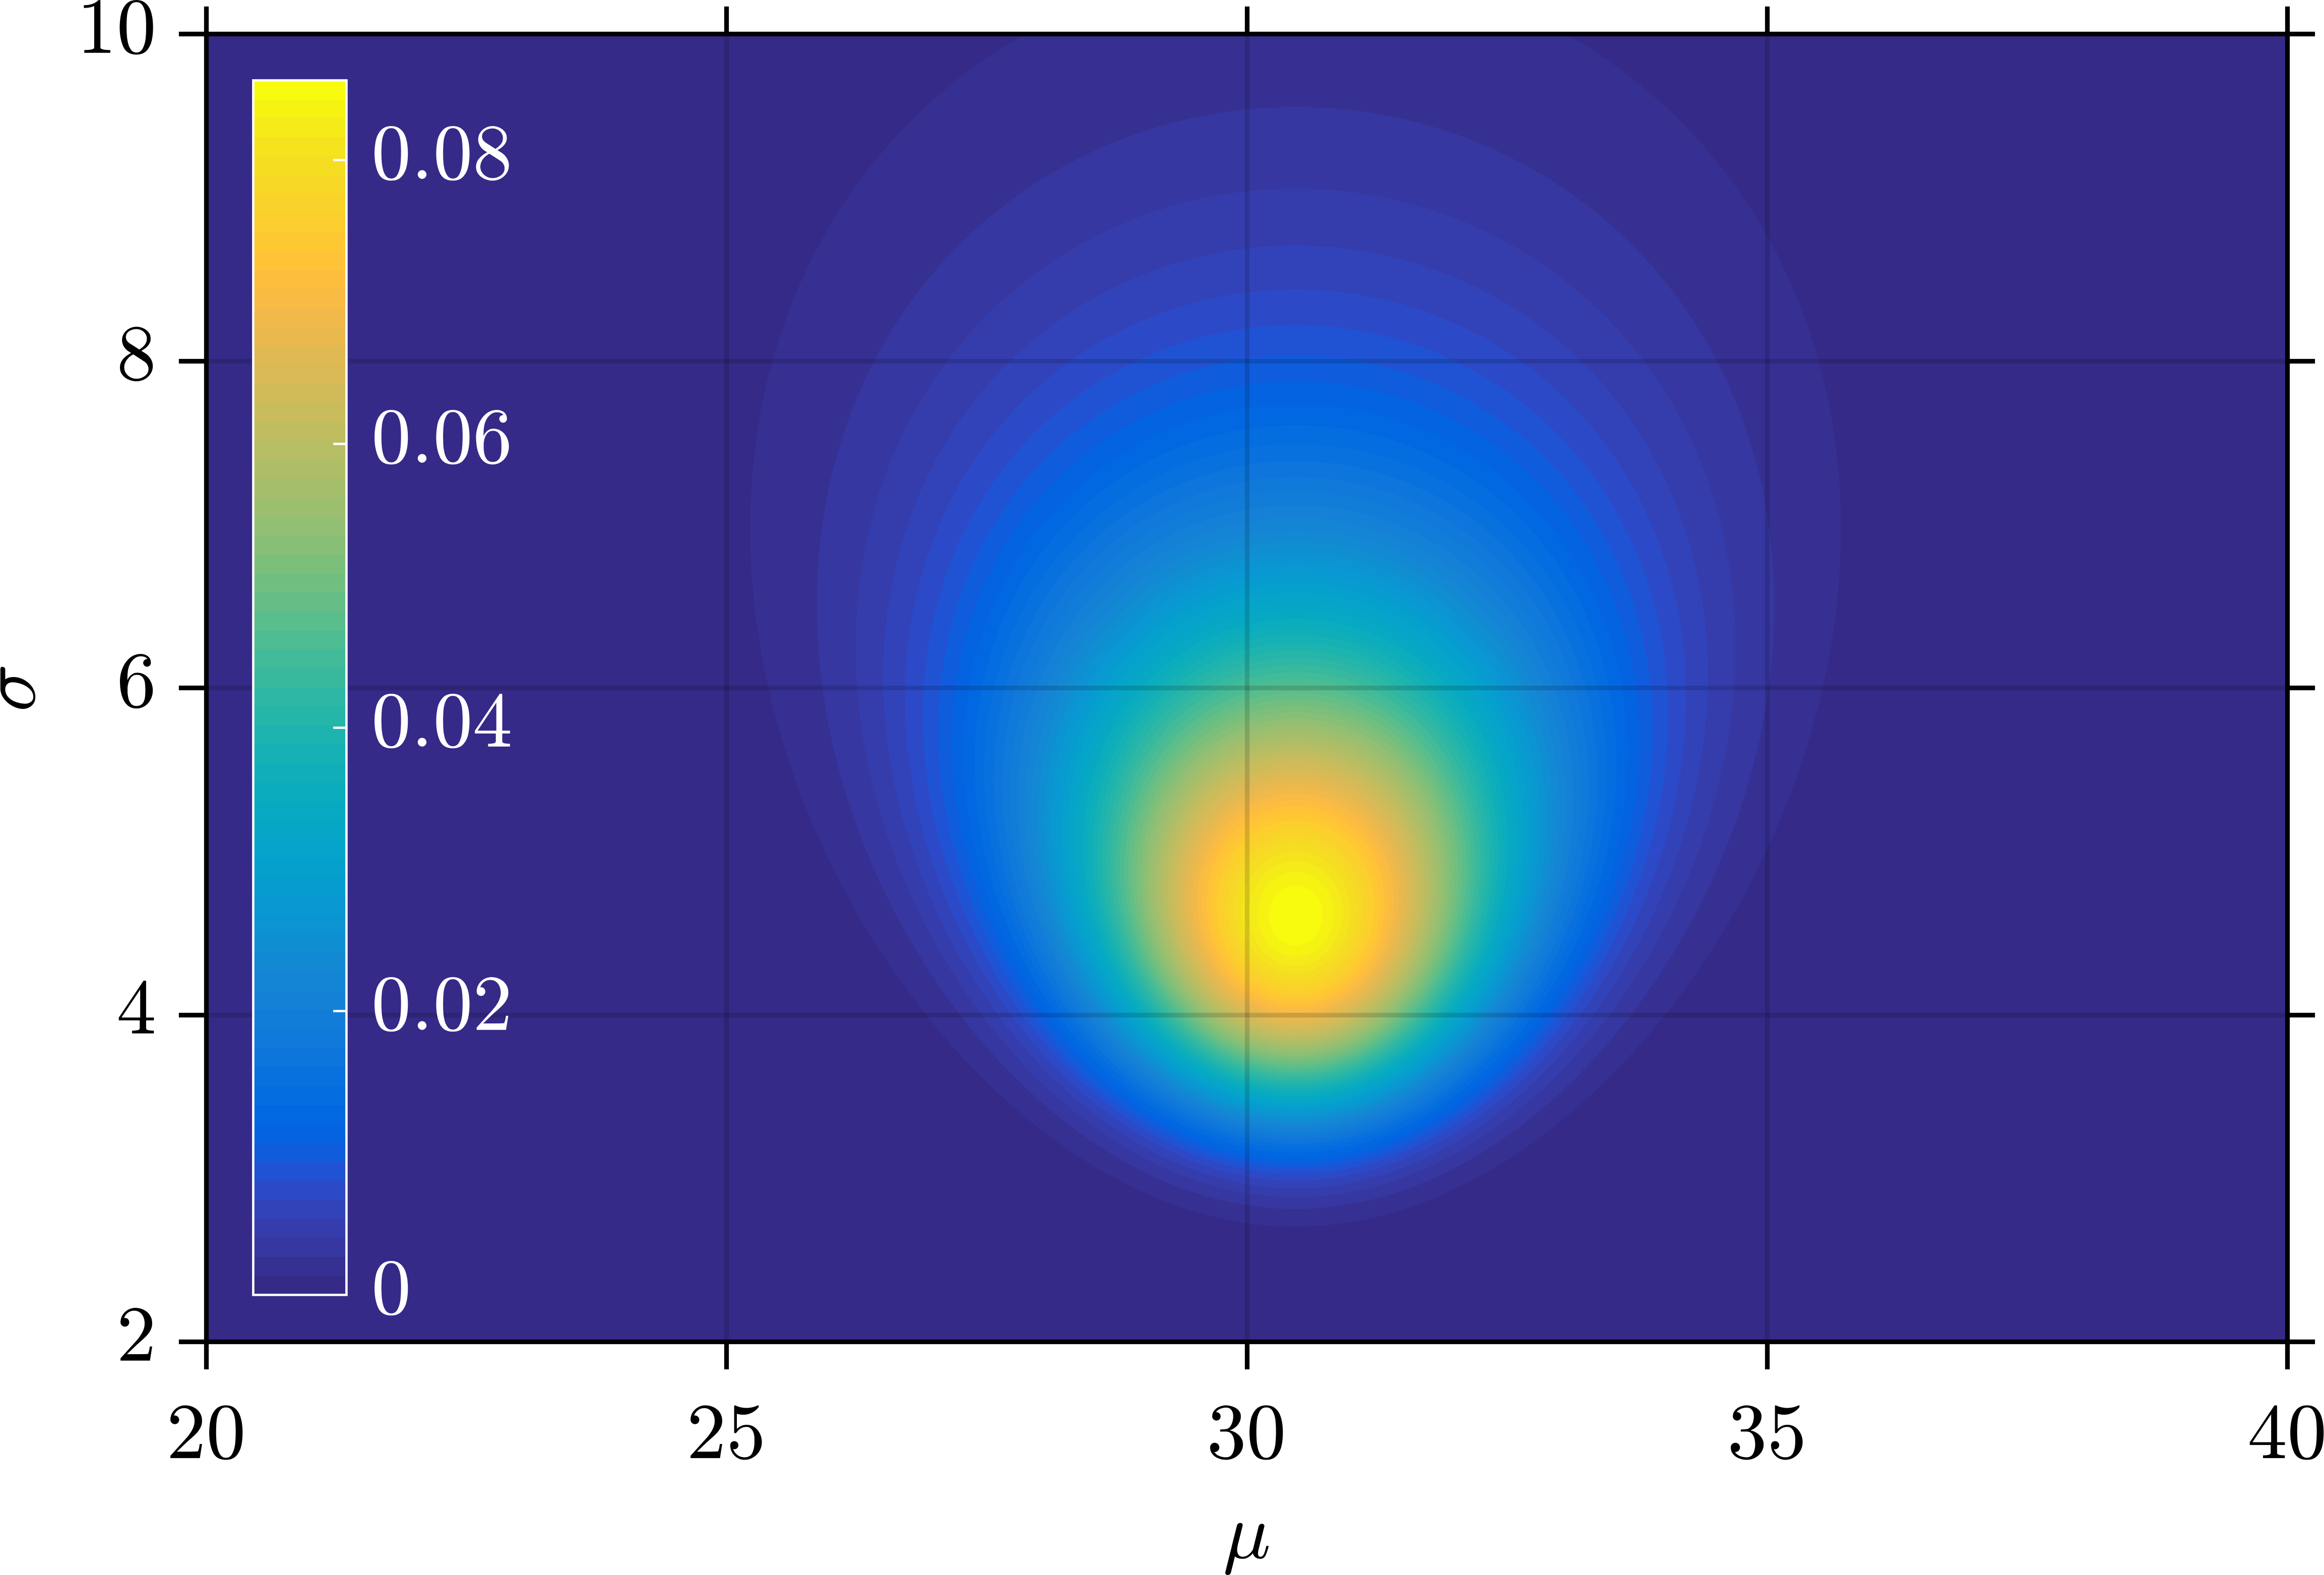
\includegraphics[height=\JCPfigHeight]{fig_JCP_Norm2D_Post2D_SLE}
    \caption{SLE with \(p = 50\).}
    \label{fig:JCP:Normal:Post2D:SLE}
  \end{subfigure}\\[1ex]%
  \begin{subfigure}[b]{\JCPsubWidth}
    \centering
    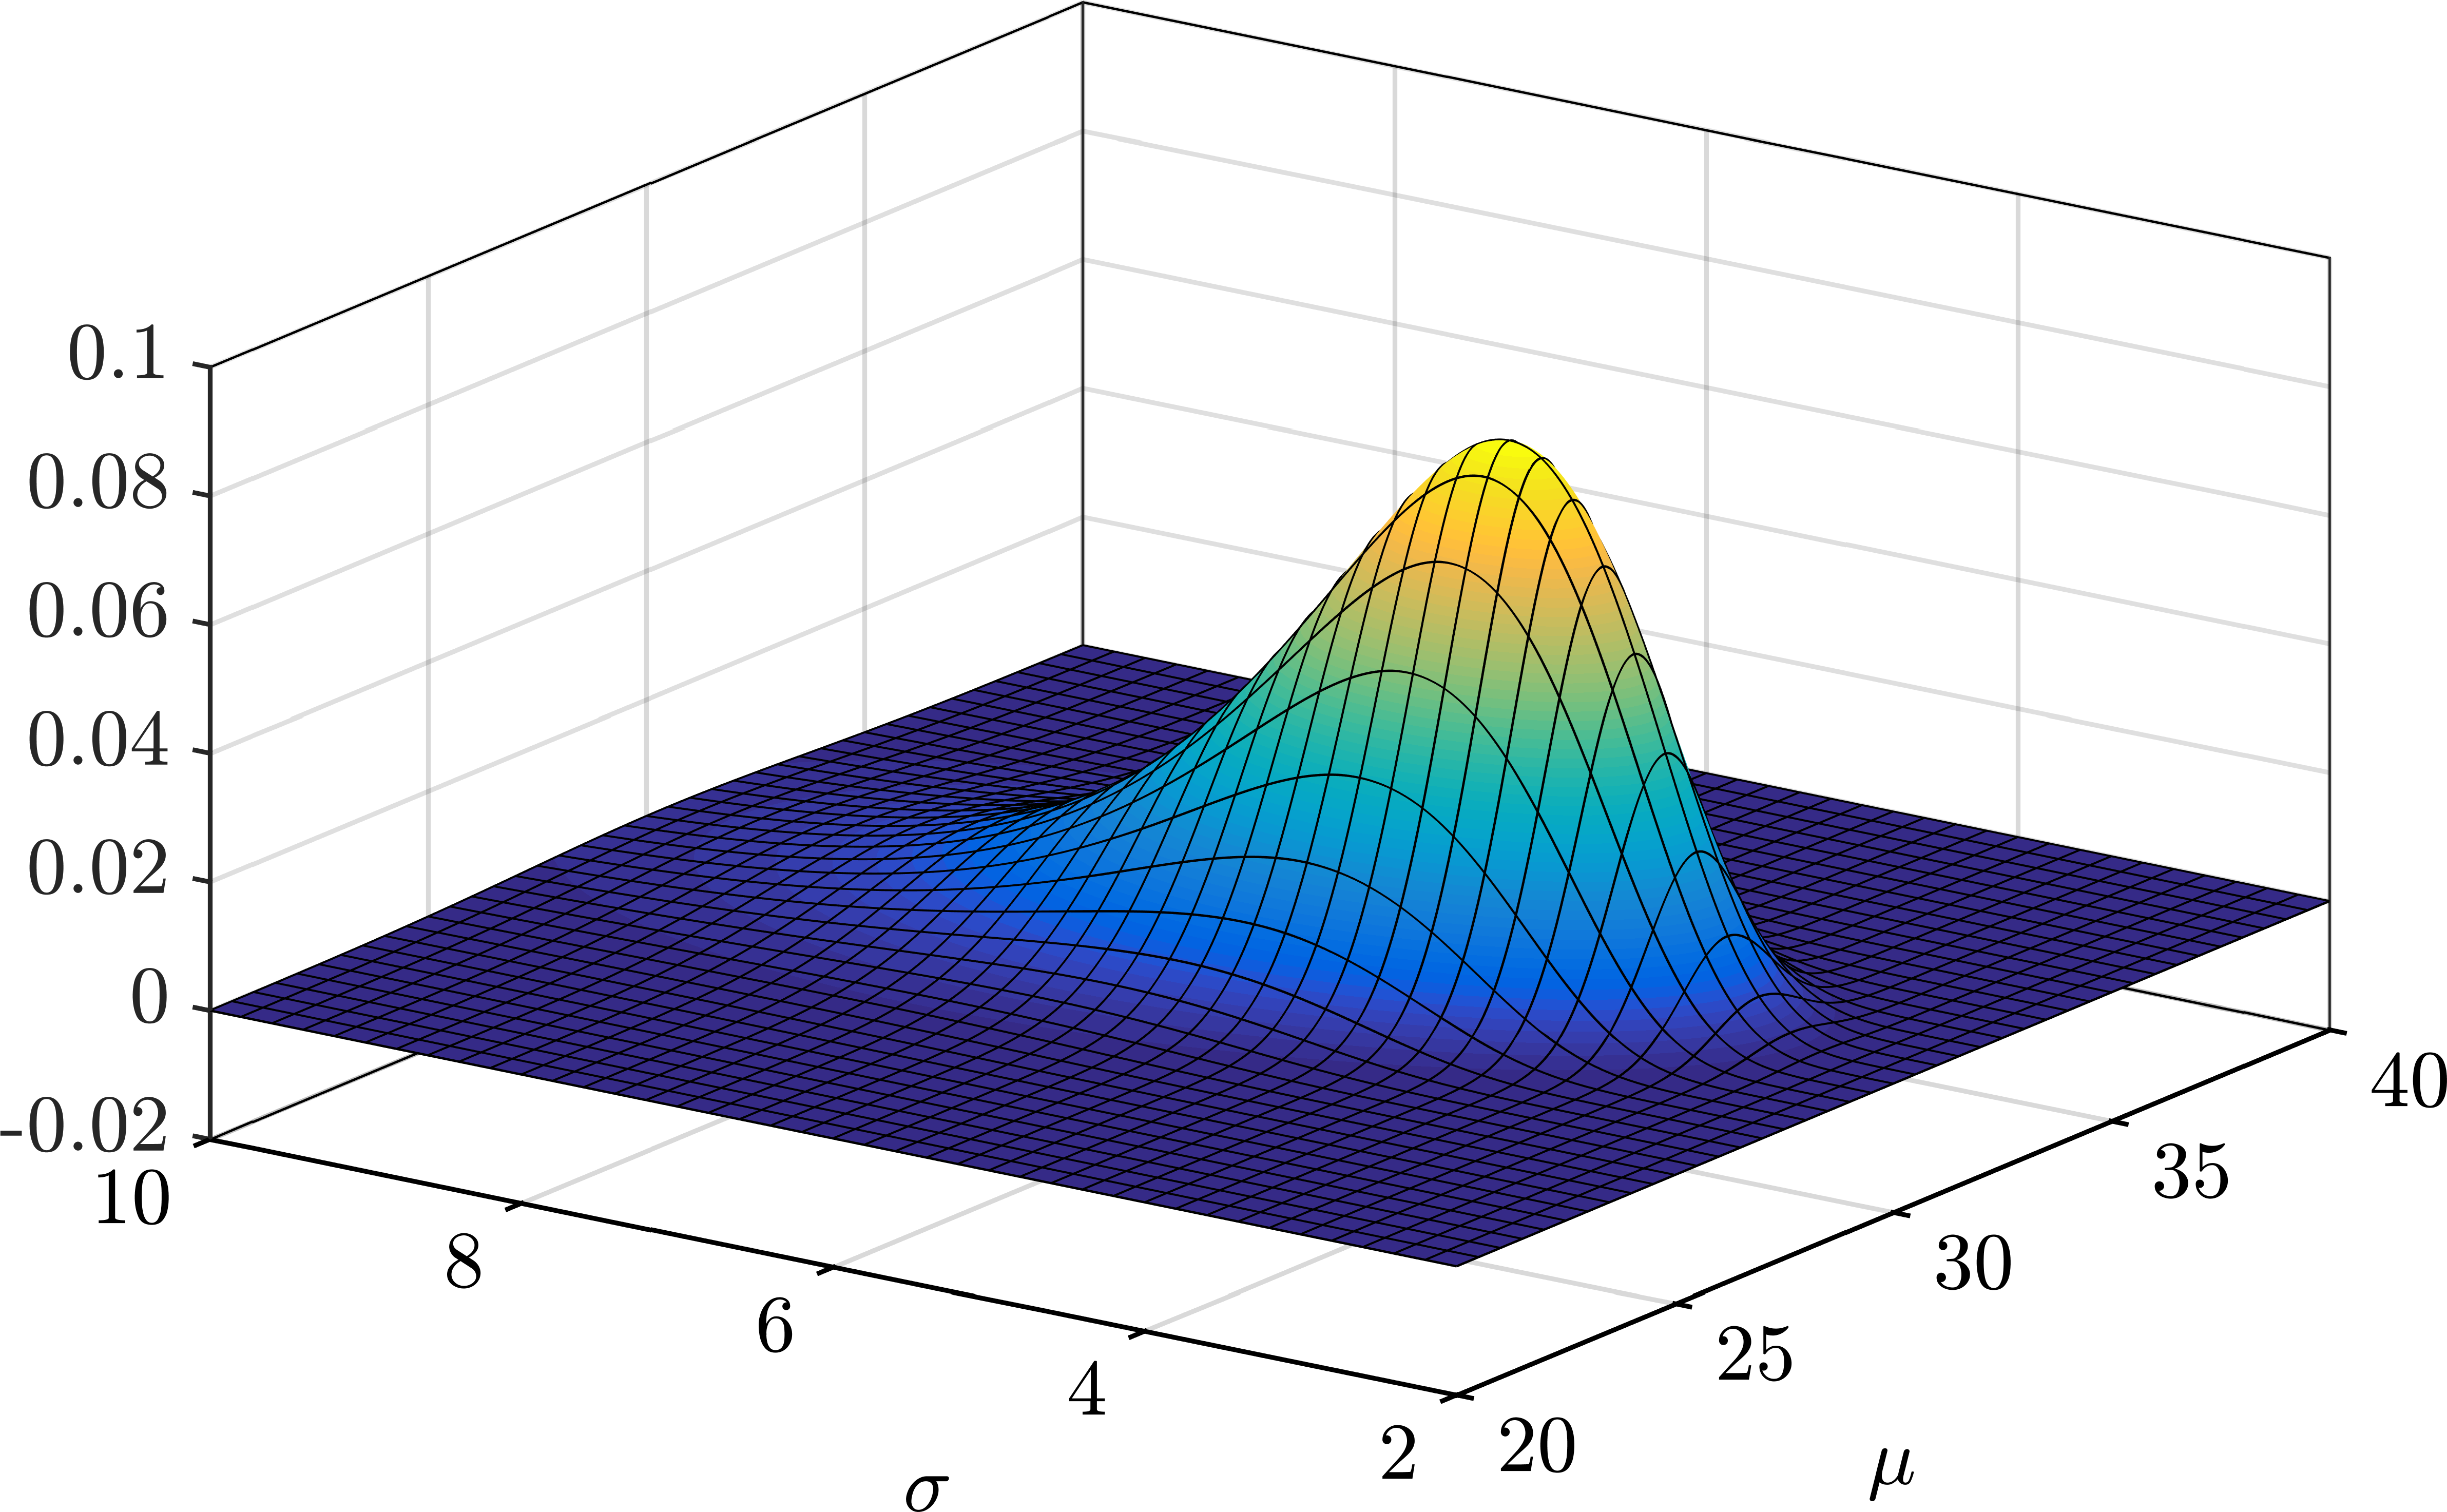
\includegraphics[width=\JCPfigWidth]{fig_JCP_Norm2D_Post3D_SLE}
    \caption{SLE with \(p = 50\).}
    \label{fig:JCP:Normal:Post3D:SLE}
  \end{subfigure}%
  \caption[2D normal fitting: Joint posterior]{2D normal fitting: Joint posterior.}
  \label{fig:JCP:Normal:Post2D}
\end{figure}
\par % POSTERIOR MARGINALS
Now the posterior marginals \(\pi(\mu \cond \bm{y})\) and \(\pi(\sigma \cond \bm{y})\) are computed from the joint posterior.
On the one hand, samples from the posterior marginals are obtained by restricting the analysis to the corresponding components of the joint MCMC sample.
On the other hand, functional approximations of the posterior marginals are extracted based on sub-expansions \(\hat{\mathcal{L}}_{\mu,p}(\mu)\)
and \(\hat{\mathcal{L}}_{\sigma,p}(\sigma)\) of a joint SLE \(\hat{\mathcal{L}}_p(\mu,\sigma)\) as in \cref{eq:JCP:SLE:Marginal1D,eq:JCP:SLE:SubExpansion1D}.
For the SLEs with \(p = 9\) and \(p = 50\) the results are visualized in \cref{fig:JCP:Normal:Post1D}.
Histogram-based MCMC sample representations and functional SLE approximations of the marginal densities are shown, too.
As it can be seen, the marginal posteriors as obtained by MCMC and the SLE with \(p = 50\) exactly match each other.
For \(p = 9\) the posteriors marginals display some wavelike fluctuations in their tails.
% FIGURES: POSTERIOR MARGINALS
\begin{figure}[htbp]
  \centering
  \begin{subfigure}[b]{\JCPsubWidth}
    \centering
    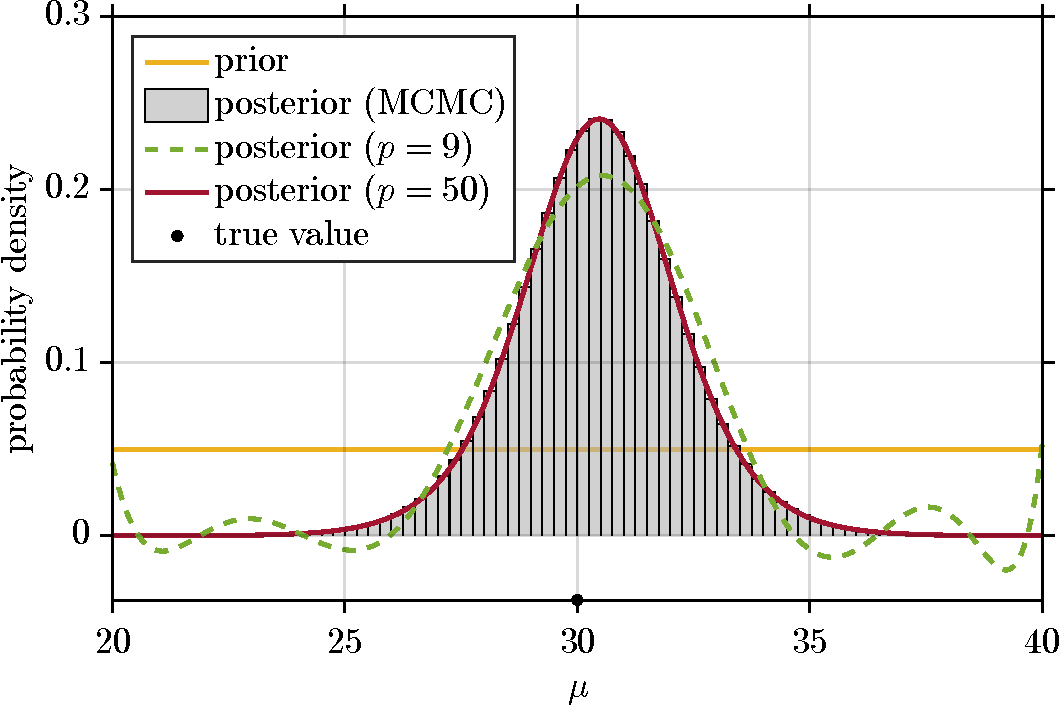
\includegraphics[height=\JCPfigHeight]{fig_JCP_Norm2D_Post1D_mu}
    \caption{Mean value \(\mu\).}
    \label{fig:JCP:Normal:Post1D:mu}
  \end{subfigure}\hfill%
  \begin{subfigure}[b]{\JCPsubWidth}
    \centering
    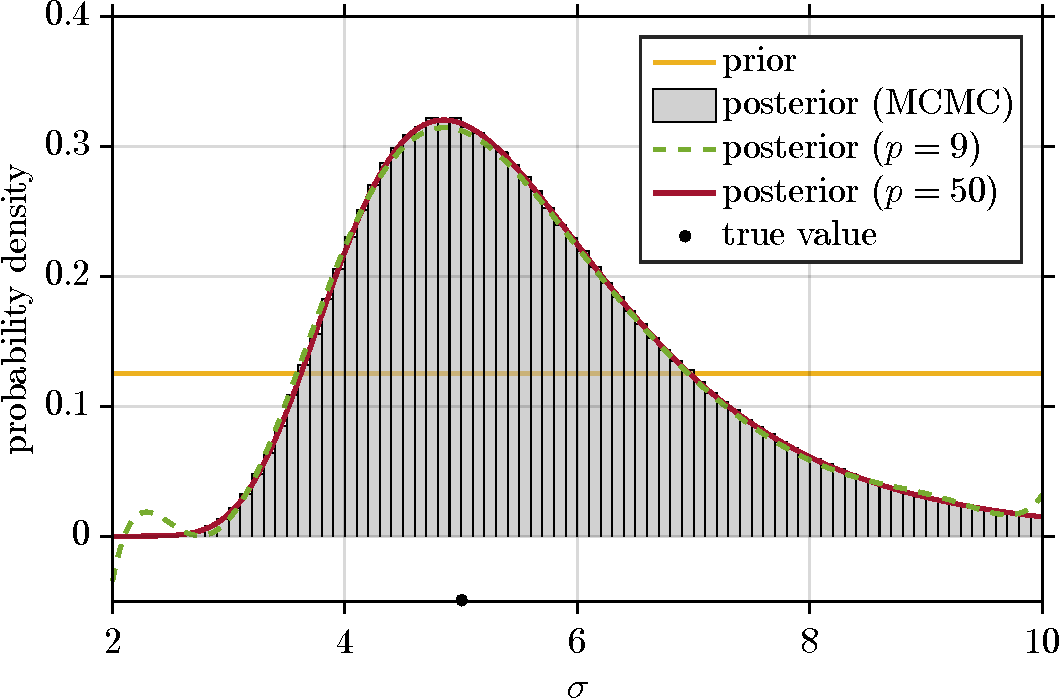
\includegraphics[height=\JCPfigHeight]{fig_JCP_Norm2D_Post1D_sigma}
    \caption{Standard deviation \(\sigma\).}
    \label{fig:JCP:Normal:Post1D:sigma}
  \end{subfigure}%
  \caption[2D normal fitting: Posterior marginals]{2D normal fitting: Posterior marginals.}
  \label{fig:JCP:Normal:Post1D}
\end{figure}

\subsubsection{Quantities of interest}
% STATISTICAL QUANTITIES OF INTEREST
Since the posterior density itself is of little inferential use, the model evidence and the first posterior moments are computed
for a selection of SLEs with varying size of the experimental design \(K\) and degree \(p\).
According to \cref{eq:JCP:SLE:ScaleFactor,eq:JCP:SLE:PosteriorMargMean,eq:JCP:SLE:PosteriorMargVariance,eq:JCP:SLE:PosteriorCovariance},
the SLE estimates of these quantities are obtained from the expansions coefficients.
In \cref{tab:JCP:Normal:StatisticalQuantities} a summary of the results is given.
Compliant with \cref{eq:JCP:SLE:ScaleFactor} the SLE estimates of the model evidence \(\scale\) are obtained as the coefficient of the constant expansion term.
According to \cref{eq:JCP:SLE:PosteriorMargMean,eq:JCP:SLE:PosteriorMargVariance}, the SLE estimates of the posterior mean \(\mathds{E}[\mu \cond \bm{y}]\)
and the standard deviation \(\mathrm{Std}[\mu \cond \bm{y}] = \mathrm{Var}[\mu \cond \bm{y}]^{1/2}\) of the location parameter \(\mu\) are computed.
Likewise, the corresponding estimates for the spread parameter \(\sigma\) follow through a simple postprocessing of the low-order expansion coefficients.
The SLE estimates of the linear coefficient of correlation
\(\rho[\mu,\sigma \cond \bm{y}] = \mathrm{Cov}[\mu,\sigma \cond \bm{y}] / \mathrm{Std}[\mu \cond \bm{y}] / \mathrm{Std}[\sigma \cond \bm{y}]\)
are computed based on \cref{eq:JCP:SLE:PosteriorCovariance}.
Additionally, the LOO error \(\epsilon_{\mathrm{LOO}}\) is listed to indicate the SLE prediction accuracy.
Note that all those estimates comply with the natural bounds and restrictions of the estimated quantities, e.g.\ the posterior means comply with the prior bounds.
\par % (MC)MC
For the sake of comparison, associated results are listed for the simulated MCMC sample, too.
These MCMC results are simply obtained as the corresponding sample approximations.
The reference estimate of the model evidence is obtained by crude MC simulation instead,
i.e.\ the arithmetic mean of the likelihood is computed for a number of \(10^8\) independent draws from the prior.
% DISCUSSION
It is interesting to note that the SLEs can reproduce the MCMC results for moderate experimental designs and degrees, say for \(K = 5 \times 10^3\) and \(p = 21\).
Even though a large number of input samples and a large polynomial degree is necessary to reproduce the shape of the joint posterior density,
significantly smaller experimental designs and polynomial orders suffice to reproduce the first posterior moments.
% TABLE: STATISTICAL QUANTITIES
\begin{table}[htbp]
  \caption[2D normal fitting: Statistical quantities]{2D normal fitting: Statistical quantities.}
  \label{tab:JCP:Normal:StatisticalQuantities}
  \centering
  \begin{tabular}{cccccccccc}
    \toprule
    & \(K\) & \(p\) & \(\epsilon_{\mathrm{LOO}}\)
    & \(\scale\) \([10^{-14}]\) & \(\mathds{E}[\mu \cond \bm{y}]\) & \(\mathds{E}[\sigma \cond \bm{y}]\)
    & \(\mathrm{Std}[\mu \cond \bm{y}]\) & \(\mathrm{Std}[\sigma \cond \bm{y}]\) & \(\rho[\mu,\sigma \cond \bm{y}]\) \\
    \midrule
    \multirow{6}{*}{\rotatebox[origin=c]{90}{SLE}}
    & \(5 \times 10^2\) & \(5\)  & \(4.24 \times 10^{-1}\) & \(1.19\) & \(30.34\) & \(5.57\) & \(2.03\) & \(1.39\) & \(\phantom{-}0.18\) \\
    & \(1 \times 10^3\) & \(9\)  & \(1.19 \times 10^{-1}\) & \(1.20\) & \(30.39\) & \(5.54\) & \(2.01\) & \(1.41\) & \(\phantom{-}0.08\) \\
    & \(5 \times 10^3\) & \(21\) & \(9.64 \times 10^{-4}\) & \(1.18\) & \(30.48\) & \(5.56\) & \(1.79\) & \(1.38\) & \(-0.01\) \\
    & \(1 \times 10^4\) & \(32\) & \(5.86 \times 10^{-6}\) & \(1.18\) & \(30.47\) & \(5.56\) & \(1.81\) & \(1.38\) & \(\phantom{-}0.00\) \\
    & \(5 \times 10^4\) & \(45\) & \(1.30 \times 10^{-9}\) & \(1.18\) & \(30.47\) & \(5.56\) & \(1.81\) & \(1.38\) & \(-0.00\) \\
    & \(1 \times 10^5\) & \(50\) & \(\phantom{^{1}}6.05 \times 10^{-11}\) & \(1.18\) & \(30.47\) & \(5.56\) & \(1.81\) & \(1.38\) & \(-0.00\) \\
    \midrule
    \multicolumn{4}{c}{(MC)MC}                             & \(1.18\) & \(30.47\) & \(5.56\) & \(1.81\) & \(1.38\) & \(-0.00\) \\
    \bottomrule
  \end{tabular}
\end{table}